%%
%% OpenMP.tex
%% Login : <hoang-trong@hoang-trong-laptop>
%% Started on  Wed Jul 29 23:28:50 2009 Hoang-Trong Minh Tuan
%% $Id$
%% 
%% Copyright (C) 2009 Hoang-Trong Minh Tuan
%%

\chapter{OpenMP}
\label{chap:openmp}


\href{http://www.open-mpi.org/}{OpenMP} is a new MPI project that was
specifically designed for shared-memory-space (multicore or SMP
machine). OpenMP particularly fits ``high-end workstations rather than
supercomputer for complex computational applications''[NYT 28Oct,
1997]. OpenMP has
\begin{enumerate}
\item some compiler directives $\rightarrow$ help compiler generate
  more efficient code
  \begin{itemize}
  \item Fortran directives, start with \verb.!$OPENMP.
  \item C/C++ pragmas 
  \end{itemize}

\item some libraries routines
\item environment variables
\end{enumerate}
that can be used to specify the region of code that can be run in
parallel, aka {\bf parallel region}, when OpenMP is enabled.  OpenMP
is not designed to run across multiple machines like MPI. If you want
your application to be portable on both clusters and SMP machines, MPI
is the solution.  As multicore continues to grow, the number of
processors on an SMP will continue to grow.

OpenMP is a highler-level abstraction for native Pthreads
programing. At its core, OpenMP uses Pthreads, yet the details are
hidden from the programmer. Like all other higher level approaches,
OpenMP sacrifices flexibility for the ease of writing code.  OpenMP
shared-memory programming model is a collection of compiler
directives, library routines, and environment variables that can be
used to specify the shared-memory parallelism in Fortran, C, C++
programs. In our chapter, we discuss OpenMP Fortran only.


Important terminologies:
\begin{itemize}
\item {\bf Thread}:

\item {\bf Region}:

\item {\bf Parallel region}:

\item {\bf Task}: 
\end{itemize}

The definition of an {\it active parallel region} has changed between
OpenMP2.5 and 3.0. Since 3.0, an active parallel region is a parallel
region that is being executed by more than one thread; otherwise, it
is an {\it inactive parallel region}. 

Before the release of GCC 4.2, OpenMP was only available in commercial
compilers. In gcc and gfortran, OpenMP programs can be compiled using
{\bf -fopenmp} flag.

{\bf Example}: Ubiquitous matrix multiplication

\begin{verbatim}
      ! OpenMP version
$ gfortran -fopenmp -o matmult_omp matmult.f
      ! sequential version
$ gfortran -o matmult matmult.f    
\end{verbatim}
To test the running time
\begin{verbatim}
$time ./matmult

$ time ./matmult_omp
\end{verbatim}

PGI compiler currently supports only ONE level of parallel, e.g. NO
support for nested parallel region. Thus, \verb!OMP_NESTED! should not
be changed.

There is an environment variable called OMP\_NUM\_THREADS that will tell
OpenMP binaries how many threads to use. If this is not defined, one
thread per CPU (core) is used. Using more threads than the available
CPUs or cores, can make the program run slower.

\section{Directives}
\label{sec:directives}

OpenMP directives mark the region of code that should be run in
parallel. The program should be compiled with
\begin{itemize}
\item PGI Fortran: ``mpif90'', or ``mpf95 -mp''
\item GCC:
\item Intel Fortran: ...
\end{itemize}

OpenMP Fortran directives (or Fortran parallelization directives) has
the form\footnote{\url{https://computing.llnl.gov/tutorials/openMP/}}
\begin{verbatim}
sentinel directive-name [clause]
\end{verbatim}
The \textcolor{red}{sentinel} should be separated with the
directive-name by at least one white space.  In fixed-form source,
\verb!sentinel! can be either
\begin{verbatim}
!$OMP , C$OMP, or *$OMP
\end{verbatim}
and \textcolor{red}{starting at column 1}. In free-form source,
\verb!sentinel! must be \verb.!$OMP..

The directive can extend multiple line using an ampersand (\&) at the
end of the line (free-source form) or a non-blank character on the
fifth column of the continuous line (fixed-source form).

\begin{lstlisting}
!!! free-source form
!$OMP PARALLEL DEFAULT(NONE) SHARED(A, B) PRIVATE(C, D) &
!$OMP REDUCTION(+:A)

!!! fixed-source form
!$OMP PARALLEL DEFAULT(NONE) SHARED(A, B) PRIVATE(C, D) 
!$OMPx REDUCTION(+:A)
\end{lstlisting}

The \textcolor{red}{directive-name} can be any of the following
directives, as shown in Table \ref{tab:OpenMP_Fortran_directive}. The
valid clause depend on the directive-name being used.
\begin{table}[hbt]
\begin{center}
\caption{Fortran directive-names for OpenMP}
\begin{tabular}{cl} 
\hline
Directive-name & Explanation \\ 
\hline\hline
BARRIER & specify the point at which all thread should be \\
 & synchronized, i.e. all threads have to complete \\
 & their works before any of them can continue \\
CRITICAL ... END CRITICAL & define the region, inside a parallel
region, \\
   & that should be run by a single thread only \\
MASTER ... END MASTER & specify the code that should be \\
      & on the master thread only \\
PARALLEL DO & a short cut for PARALLEL ... END PARALLEL region \\
     & that contains only a single DO directive right after \\
     & the line of PARALLEL directive \\
DO ... END DO & divide and distribute this region to all available \\
          & threads to run in parallel \\
PARALLEL ... END PARALLEL & define a {\it parallel region} within which \\
   & you can define a parallel directives. Then, the region is
   executed\\
   & by only a single thread, until it reachs this parallel
   directive\\

\end{tabular}
\end{center}
\label{tab:OpenMP_Fortran_directive}
\end{table}

As you can see, several OpenMP Fortran directives come in pairs and
have the form below
\begin{verbatim}
!$OMP  directive 

    [ structured block of code ]

!$OMP END  directive
\end{verbatim}

Such directives allow programmers to
\begin{itemize}
\item create task,
\item create loop, and 
\item create parallel section work-sharing
constructs and synchronization constructs. 
\item define how data is shared or copied between parallel threads of
  execution.
\end{itemize}

Among all directives, the most important directives is the one in
charge of defining the so-called {\bf parallel region}; that is
\verb.!$OMP PARALLLEL/!$OMP END PARALLEL. The equivalent form is the
single \verb.!$OMP PARALLEL DO. that must be followed by a DO loop.

\begin{itemize}
\item To learn how to use  OpenMP directives with your codes, read
\hyperref[sec:tasks]{Task}. 

\item To learn how many threads are being used, read the Section
\ref{sec:openmp-statements}
%\ref{sec:envir-vari}.

\end{itemize}

References:
\begin{itemize}
\item \url{http://www.atnf.csiro.au/computing/software/sol2docs/mr/READMEs/openmp.html}
\end{itemize}

\section{OpenMP statements}
\label{sec:openmp-statements}

OpenMP also define a set of routines. To specify that a statement that
use these routine being compiled only for OpenMP-compliant compilers,
you can put \verb.!$. in front of the statement.
\begin{lstlisting}
!$ interval = L * OMP_get_thread_num() / &
!$ (OMP_get_num_threads() - 1)
\end{lstlisting}

% \section{Libraries Routines}
% \label{sec:libraries-routines}
There are rountines that can query the runtime enviroment, e.g. to
determine the number of thread are participating in the execution of a
parallel region of code. 
% \section{Environment variables}
% \label{sec:envir-vari}
The performance of a parallel program is heavily determined by the
number of threads. This and many other information can be given to the
program via using an appropriate routines, or by default, are
specified in environment variables.

In Fortran, this can be done via
\begin{lstlisting}
CALL OMP_SET_NUM_THREADS(4)
\end{lstlisting}
To set any of the below environment variable, use
\begin{verbatim}
setenv OMP_SCHEDULE "STATIC, 5"
\end{verbatim}
or read section~\ref{sec:set-envir-vari}.

In general, we need to set \verb!OMP_NUM_THREADS! to a value no larger
than the available number of processors on the target platform. Set
\verb!OMP_DYNAMIC!  to FALSE to use the number of threads specified by
\verb!OMP_NUM_THREADS!.
 

\section{Mechanism}
\label{sec:mechanism}

Before or after a parallel region, the code is executed by only one
thread. This is the way that traditional program executes, aka serial
program. Thus, these regions are called {\bf serial regions}. The
thread that execute the serial regions is called the
{\bf master thread}. When a parallel region is detected, the master
thread create a set of threads, called {\bf slave threads}, to run the
parallel region concurrently. The master thread can also join into the
computation like any slave threads. 

Each slave thread has a unique {\bf thread number} ranging from zero
to $N_p-1$ with $N_p$ is the number of threads (probably including the
master thread if it join in the computation).

There are many information that a programmer can specify how the
parallel region is executed
\begin{enumerate}
\item the scopes of variables
\item the number of threads
\item special treatments of some variables
\item ...
\end{enumerate}
These are specified in a set of clauses 
\begin{lstlisting}
!$OMP directive clause1 clause2 ...
\end{lstlisting}
Depending on the directive, we can have different clauses.

\section{PARALLEL region}
\label{sec:parallel-region}

There can be only ONE work-sharing construct only for a PARALLEL
region. It is aka {\bf combined parallel work-sharing
  constructs}. This region can be defined by one of the two directives
\begin{lstlisting}
!(1)
!$OMP PARALLEL DO clause1 clause2 ...
  DO ...

!(2)
!$OMP PARALLEL clause1 clause2
  DO ...
!$OMP END PARALLEL
\end{lstlisting}
After PARALLEL DO must be a DO loop, yet within PARALLEL/END PARALLEL
pair, it can be anything. \verb.!$OMP END PARALLEL. has an implicit
synchronization, i.e. wait until all thread complete before returning
the control to the master thread.

The clauses that we can use for PARALLEL region are
\begin{enumerate}
\item PRIVATE(list): declare a list of variables that are local to
  each thread.
\item SHARE(list)
\item DEFAULT(PRIVATE | SHARED | NONE)
\item FIRSTPRIVATE(list)
\item COPYIN(list)
\item REDUCTION(operator:list)
\item IF(\verb.scalar_logical_expression.)
\item \verb.NUM_THREADS(scalar_integer_expression).: specify the
  number of threads to process the parallel region. 
\end{enumerate}

It is possible to nest parallel regions into parallel regions. 
\begin{lstlisting}
!$OMP PARALLEL 
   ...
   !$OMP PARALLEL
   ...
   !$OMP END PARALLEL
   ...
!$OMP END PARALLEL
\end{lstlisting}
\begin{figure}[hbt]
  \centerline{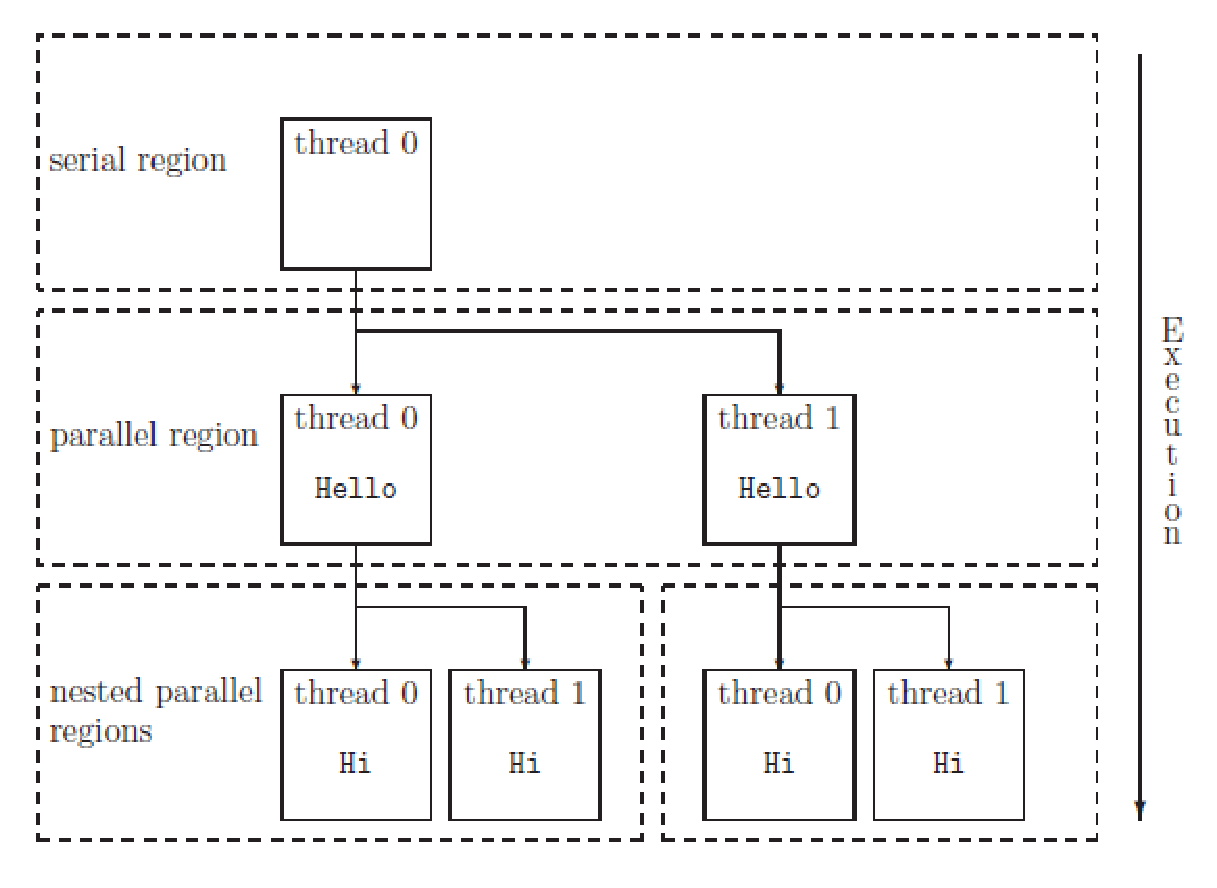
\includegraphics[height=5cm,
    angle=0]{./images/nested_parallel_region.eps}}
\caption{Execution of nested parallel regions}
\label{fig:nested_parallel_reg}
\end{figure}

\section{Clauses}
\label{sec:clauses-1}

There are two types of clauses: {\bf data scope attribute clauses}
(specify how each variable is handled and which thread is allowed to
see its value and change it), the second type involves all clauses
that don't fit to the first type. 

\subsection{PRIVATE}
\label{sec:private}

A variable should have different values in each thread, then you
specify it in the PRIVATE clauses
\begin{lstlisting}
!$OMP PARALLEL PRIVATE(a, b)
\end{lstlisting}
with $a, b$ are two variables. Variables declared as private have an
undefined value at the peginning of the parallel region. The variables
like counters for DO-loop, FORALL command, or implicit DO-loop or any
one that are specified to be THREADPRIVATE become private
automatically to each thread. 


\section{Tasks}
\label{sec:tasks}

Let's make yourself familiar with this concept: task. Any part of your
code can be considered as a task. Here are the properties of a task,
it has
\begin{enumerate}
\item  some code to execute
\item  its own data
\item  an assigned thread to execute that code and use the data
\end{enumerate}

\subsection{Task construct}
\label{sec:task-construct}

A task construct is a {\it task directive} plus a structured block 
\begin{verbatim}
#pragma omp task [clause[[,]clause] ...]
{       
    structured-block
}
\end{verbatim}
you can have one or more  \verb!clause! which can be one of the
following
\begin{verbatim}
if (expression)
untied
shared (list)
private (list)
firstprivate (list)
default( shared | none )
\end{verbatim}



\subsection{Task scheduling}
\label{sec:task-scheduling}




\section{Write to shared-data}
\label{sec:write-shared-data}

Simultaneous write to a shared containers must be protected by 
\begin{verbatim}
#pragma omp critical
\end{verbatim}
section.

\section{Parallel a DO loop}
\label{sec:parallel-do-loop}

A DO loop is very common. Then, the question is ``do we always be able
to parallelize a DO loop?'' - The answer is NO.

This is an example of DO loop in which the execution of one loop is
independent from the other.
\begin{lstlisting}
DO i=1, 10
  A(i) = i
END
\end{lstlisting}
Here, the computation of A(i) and A(i+1) are independent.

However, let's learn all possible cases.  Here is a classification of
data dependencies\footnote{\url{http://www.ibiblio.org/pub/languages/fortran/ch2-17.html}}
\begin{verbatim}
 ------------------------------
 The dependencies we will discuss are: 

    Store before load      Competing stores      Load before store
    =================      ================      ===============
    DO I=2,4               DO I=2,4              DO I=2,4        
      A(I-1) = B(I)          A(I-1) = B(I)         B(I) = A(I-1) 
      C(I)   = A(I)          A(I)   = C(I)         A(I) = C(I)   
    ENDDO                  ENDDO                 ENDDO           

    Recurrence             Sum reduction
    ===============        ==============
    DO I=2,4               SUM = 0.0
      A(I) = A(I-1)        DO I=2,4
    ENDDO                    SUM = SUM + A(I)
                           ENDDO
\end{verbatim}

\subsection{Store before hand}
\label{sec:store-before-hand}

A technique called PRE-LOADING can make the code parallelable.
\begin{lstlisting}
      DO I=2,4
        TEMP   = A(I)
        A(I-1) = B(I)
        C(I)   = TEMP
      ENDDO
\end{lstlisting}

\subsection{Recurrence}
\label{sec:recurrence}

This situation, the dependency is essential and cannot be removable.
\begin{lstlisting}
      DO I=2,4          
        A(I) = A(I-1)   
      ENDDO            
\end{lstlisting}

\section{Choice of number of threads}
\label{sec:choice-numb-thre}

When you set \verb!OMP_NUM_THREADS!, you over-ride any relationship
between the number of processors and the number of threads chosen by
OpenMP. If you set more threads than processors, you have threads
waiting for an opportunity to run. You would expect performance to
degrade when you choose too many
threads\footnote{\url{http://software.intel.com/en-us/forums/threading-on-intel-parallel-architectures/topic/47535/}}.

If you do any reading about threading or OpenMP, you will see there
are several common problems which could block speedup by threaded
parallelism. If it were not so, there wouldn't be justification for
supporting tools such as Intel Thread Profiler.

OpenMP compilers generally don't pay any attention to false sharing,
even in simple cases where it might be possible to diagnose. On modern
processors which have significant Instruction Level Parallelism when
running a single thread, you could easily find ways to defeat ILP with
threaded parallelism. These ideas hardly make a dent in the list of
possibilities.


\section{How to compile a program}
\label{sec:how-compile-program}

\begin{enumerate}
\item PGI: pgf95 (Fortran 90/95), pgf77 (FORTRAN 77)
\end{enumerate}
\subsection{PGI compiler}
\label{sec:pgi-compiler}

In the makefile, add the \verb!-mp! switch to FFLAGS variable to
enable processing of OMP pragmas 


\section{How to run a program}
\label{sec:how-run-program}

code, see ''Parallel Programming Using PGI Compilers'' in the PGI User's
Guide.

\section{In C/C++}
\label{sec:cc++}

\subsection{Pragmas}
\label{sec:pragmas}

Pragmas is a dialect to directives and is a technical term in C/C++
programming language. Pragmas is not covered here. However, you should
know a pragmas for OpenMP begins with
\begin{verbatim}
#pragmas omp
\end{verbatim}



%%% Local Variables: 
%%% mode: latex
%%% TeX-master: "gpucomputing"
%%% End: 
